%!TEX root = ../../../../memoria.tex
\subsection{Opciones de \ShippingCOM}\label{chapter:solucionimplementada:section:shipping_options}

	Como se describió en la sección \nameref{cap:solucionImplementada:section:dashboard:subsection:shipping} (\ref{cap:solucionImplementada:section:dashboard:subsection:shipping}) la implementación de \ShippingCOM ha sido simplificada considerablemente. Sin embargo, la implementación existente permite la elección entre diferentes métodos de \ShippingCOM previamente definidos (\refFigura{figure:shipping:checkout:select_option}). 

	\begin{figure}[H]
		\centering
		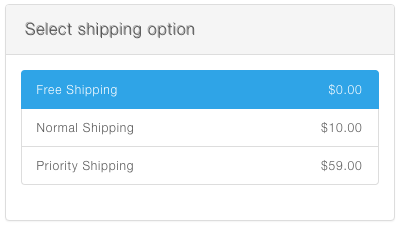
\includegraphics[width=0.7\textwidth]{figuras/checkout/shipping_options.png}
		\caption{Opcions de \shippingEF configuradas en el sistema.}
		\label{figure:shipping:checkout:select_option}
	\end{figure}

	En caso de no tener ningún método de \shippingEF disponible, o si el \packageAS a sido deshabilitado, entonces aparecerá un mensaje ( \refFigura{figure:shipping:checkout:shipping_methods_unavailable}) que indicará que no hay métodos disponibles.

	\begin{figure}[H]
		\centering
		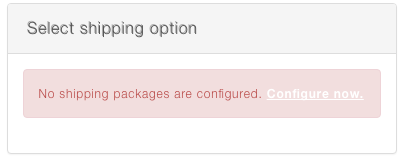
\includegraphics[width=0.6\textwidth]{figuras/checkout/shipping_methods_unavailable.png}
		\caption{Mensaje cuando no hay opciones de \shippingEF configuradas en el sistema.}
		\label{figure:shipping:checkout:shipping_methods_unavailable}
	\end{figure}